\documentclass[aps,pra,twocolumn]{revtex4-1}

\usepackage{graphicx,epstopdf}
\usepackage{amsmath}
\usepackage{mathrsfs}
\usepackage{mathtools}


\begin{document}


\title{Determination of the drag coefficient of an ARO89019 mirage rocket}

\author{Evan Anders}
\author{Andrew French}
\author{John Hoff}
\author{Michael Woodkey}
\affiliation{Department of Physics, Whitworth University, 300 W. Hawthorne Rd., Spokane, WA 99251}


\date{\today}

\begin{abstract}
Here we derive equations of motion for the flight of a rocket which experiences a quadratic drag force.  Using these equations as a model, we utilize $\chi^2$ minimization techniques to determine the drag coefficient of a mirage ARO89019 rocket.  We find the drag coefficient of the rocket to be $\gamma = 1.21$ kg/m$^3$.
\end{abstract}



\maketitle


\section{\label{section1} Introduction}
In introductory physics we learned to model projectile motion using initial velocities and gravitational acceleration.  In advanced dynamics, we have improved upon this model by accounting for linear and quadratic drag forces.  It is our goal to verify the correctness of these drag forces using real altitude data from the flight of a Mirage ARO89019 rocket propelled by an Aerotech g38 motor.  In verifying the efficacy of the drag model, we will determine the drag coefficient of the rocket.  In section \ref{section 2}, we will examine the equations of motion for a flying rocket.  In section \ref{section 3}, we will discuss motor calibration.  We discuss data analysis techniques and our best-fit value of the drag coefficient in section \ref{section 4}.  A discussion of sources of error occurs in section \ref{section 5}.



\section{\label{section 2} Theory}
It is a good approximation to assume that drag forces act entirely in a direction opposite to that of velocity, where
\begin{equation}
\vec{f}_\text{drag} = - f(v) \hat{v}.
\end{equation}
At speeds relative to our experiment, we define
\begin{equation}
f(v) = f_\text{linear} + f_\text{quadratic} = b v + c v^2 ,
\end{equation}
where $f_\text{linear}$ will arise as a result of the viscous properties of air and $f_\text{quadratic}$ is caused by the projectile pushing air particles out of its path \cite{taylor2005}.  At high speeds, such as those at which rockets travel during ascent, the linear term becomes insignificant.  For a long, cylindrical object whose velocity is aligned with the area vector of the top of the cylinder, the value of the quadratic drag coefficient becomes
\begin{equation}
c = \gamma A = \gamma \pi r^2,
\end{equation}
where $r$ is the radius of the cylinder and $\gamma$ is a constant with units of mass/volume determined by the body in motion.

The equation of motion for such a moving body subject to gravity and drag is \cite{taylor2005}
\begin{equation}
m \dot{\vec{v}} = m \vec{g} - c v \vec{v}, \label{dragC}
\end{equation}
where $g$ is the acceleration due to gravity.  Breaking the motion of our rocket into a two-dimensional plane (horizontal $x$ and vertical $y$), our equations of motion are
\begin{equation}
m \dot{v}_x  = -c v v_x \label{xafter}
\end{equation}
and
\begin{equation}
m \dot{v}_y  = -c v v_y - mg, \label{yafter}
\end{equation}
where
\begin{equation}
v = \sqrt{v_x^2 + v_y^2} \label{vValue}
\end{equation}
and $c$ is defined by Eq. (\ref{dragC}).

This system of equations is accurate for a rocket in motion \emph{after} its motor burn is completed.  Before this time, the rocket motor provides an additional force in the direction of motion, such that
\begin{equation}
\vec{f}_\text{burn} = f_\text{burn}(t) \hat{v}.
\end{equation}
During the burn, the mass of the rocket-motor system decreases.  We model mass as a linearly decreasing function of time during the burn and constant after the burn, such that 
\begin{equation}
m(t) = 
\begin{cases}
m_\text{rocket} + m_\text{fuel}\dfrac{(t_\text{burn} - t)}{t_\text{burn}}, & \text{if } t < t_\text{burn} \\ \\
m_\text{rocket} & \text{if } t \geq t_\text{burn},
\end{cases}
\end{equation}
where $m_\text{rocket}$ is the mass of the rocket plus the empty motor, $m_\text{fuel}$ is the mass of the fuel in the motor prior to launch, and $t_\text{burn}$ is the total time of the motor burn.

Acknowledging our changing masses and forces, our equations of motion become
\begin{equation}
m(t) \dot{v}_x = 
\begin{cases}
-c v v_x +  \dfrac{v_x f_\text{burn}(t)}{ v }, & \text{if } t < t_\text{burn} \\ \\
-c v v_x, & \text{if } t \geq t_\text{burn}
\label{xmotion}
\end{cases}
\end{equation}
and
\begin{equation}
m(t) \dot{v}_y = 
\begin{cases}
-c v v_y  - m(t) g+  \dfrac{v_y f_\text{burn}(t)}{ v }, & \text{if } t < t_\text{burn} \\ \\
-c v v_y - m(t) g, & \text{if } t \geq t_\text{burn},
\label{ymotion}
\end{cases}
\end{equation}
where $c$ is defined by Eq. (\ref{dragC}) and $v$ is defined by Eq. (\ref{vValue}). 

\section{\label{section 3} Calibration}
\begin{figure} [t!]
	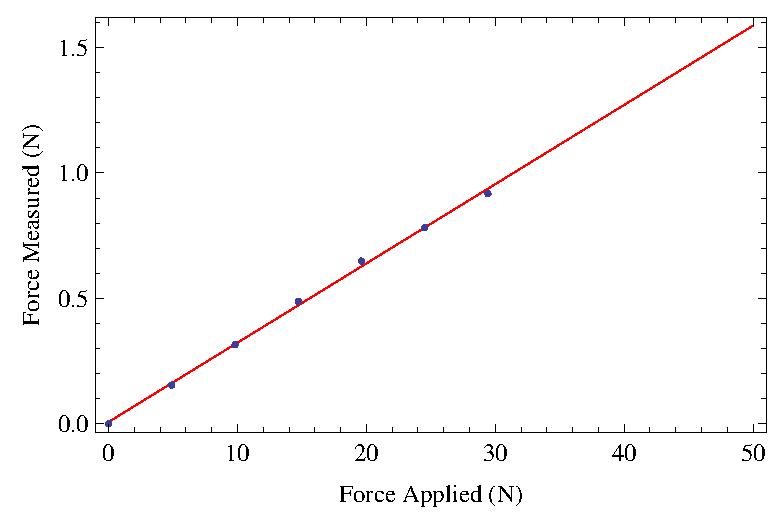
\includegraphics[width=3in]{calibration_Plot.eps}
	\caption{We hung weights from a pulley-based calibration apparatus in increments of 0.5 kg and recorded the readings of the force sensor.  Our best-fit line relating measured force and applied force is $F_\text{measured} = 0.0316F_\text{applied} + 0.00794$ N.\label{calibrationPlot}}
\end{figure}
\begin{figure} [b!]
	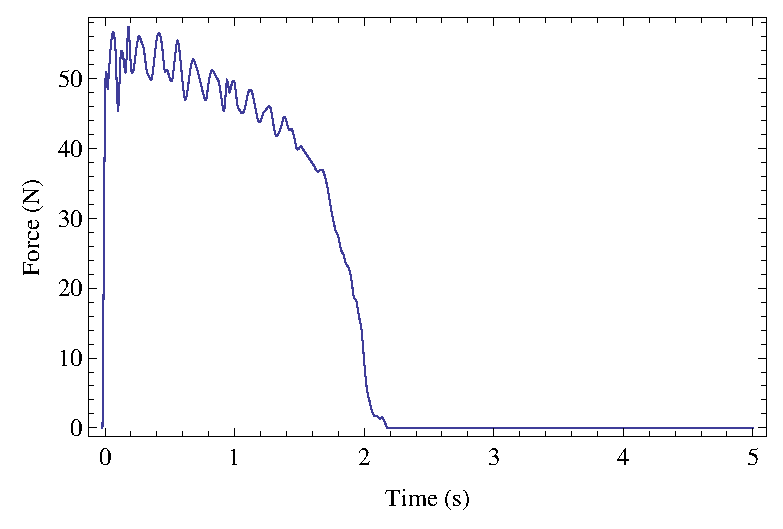
\includegraphics[width=3in]{G38-scaledTest.eps}
	\caption{The force produced by an Aerotech g38 rocket motor is shown.  Data was measured by our pulley-based calibration device and scaled by a factor of $1/0.0316$.\label{thrustPlot}}
\end{figure}

In order to calibrate the force output of our rocket motor, we crafted a pulley-based testing apparatus attached to a Vernier Dual-Range Force Sensor.  In order to determine the scaling factor between force applied to our pulley system and force measured by the sensor, we added weight to our system in increments of 0.5 kg while recording the measured force.  Results of these calibrations are shown in Fig. \ref{calibrationPlot}.   Using this data, we determined a relationship between measured force and applied force, which follows the form
\begin{equation}
F_\text{measured} = \chi F_\text{applied} + \beta,
\end{equation}
where our apparatus' force scaling factor is $\chi = 0.0316$.  A small offset, $\beta = 0.00794$ N, appeared as a result of the internal inaccuracy of our force meter and from small oscillations within the pulley system.

We used the same calibration apparatus to measure the force produced by an Aerotech g38 motor.  Applying a scaling factor of $F_\text{applied} = F_\text{measured}/0.0316$, we determined that a g38 motor fires for a total of 2.16 seconds, delivering a peak force of roughly $55$ N.  The force profile of a g38 motor is shown in Fig. \ref{thrustPlot}.



\section{\label{section 4} Experimental Data and Analysis}
The mirage flew with an on-board altimeter which measured altitude as a function of pressure.  We used Wolfram Mathematica to interpolate rocket flight altitude data recorded by the altimeter as well as our calibrated motor force data.  Utilizing Eqs. (\ref{xmotion} \& \ref{ymotion}) to describe the motion of our rocket, we employed $\chi^2$ minimization techniques to determine the best value for the drag coefficient, $\gamma$, of the mirage.

Acknowledging that our flight data showed significant noise within the first few data points after launch, we allowed our minimization routine to vary the value of initial velocity, $v_0$, between 0 m/s and 5 m/s.  Additionally, this routine varied the time-step used in gathering interpolated data, $\Delta t$, from 0.05 to 0.30 seconds.  

After setting up these parameters, we limited the data used in determining our drag coefficient to the first six seconds of data.  Although our rocket reached peak altitude shortly after seven seconds, our model fails in this regime for two reasons.  First, at peak altitude, the rocket is not traveling rapidly enough to justify ignoring the linear drag term.  Second, the rocket begins to tip; as it is no longer traveling in the direction of the nose cone, our model of $c$ in Eq. (\ref{dragC}) falls apart.

Under these conditions, the best fit obtained for the mirage's drag coefficient value was $\gamma =  1.21$ kg/m$^3$.  This value accompanied a mean deviation between our model and flight data of roughly 1.33 m per data point, where data points were taken every 0.05 s.  A comparison of this best-fit theoretical model to experimental data is shown in Fig. \ref{experiment}.

\begin{figure} [t!]
	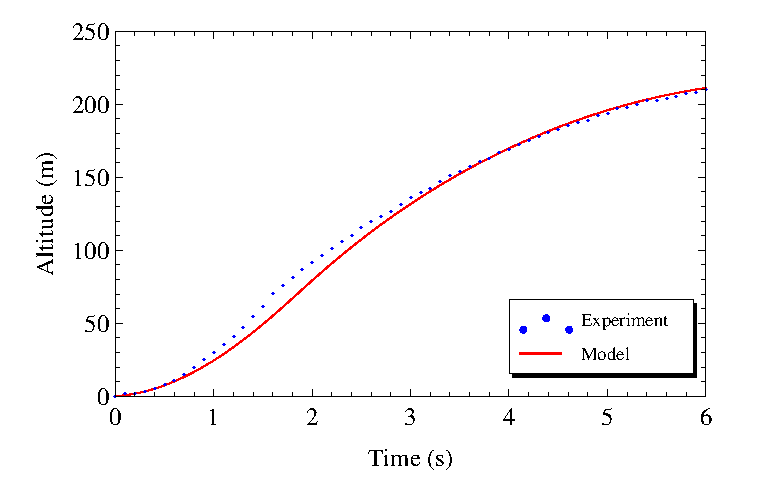
\includegraphics[width=3.5in]{Mirage-G38-BestFit.eps}
	\caption{Here we compare experimental data for the flight of a mirage with a g38 motor to our model of Eqs. (\ref{xmotion} \& \ref{ymotion}) where $\gamma = 1.21$ kg/m$^3$.  There is a mean deviation of 1.33 m between experimental and theoretical data data points.  \label{experiment}}
\end{figure}


\section{\label{section 5} Discussion}
We determined that the drag coefficient of our rocket was $\gamma = 1.21$ kg/m$^3$.  Unfortunately, this value was achieved for a model with $ v_ 0 = 5$ m/s.  While this allowance was made to account for noisy data, it is known that our rocket fired from rest. 

Once likely source of error arose from our failure to measure the launch angle of our rocket.  While our simulations ran under the assumption of a launch angle of $1^\circ$, it is probable that our launch angle was in the range of $1^\circ \pm 5^\circ$, which we did not account for in our simulations.

Additionally, while our model accounts for drag, it fails to account for wind and other small factors (such as the friction due to the launch rail).  On top of ignoring these forces, our model of the rocket as a perfect cylinder is slightly inaccurate due to the small cross-sectional area of the tail fins.

A final source of error lies in the fact that we failed to account for the oscillations introduced to our pulley system when we calibrated the g38 motor.   As seen in Fig. \ref{thrustPlot}, the force delivered by the rocket is not a smooth line, but rather an oscillation of roughly 5-10 N peak-to-peak.  These fluctuations certainly affected the interpolated values of our motor thrust.

Despite all of these error sources, our theoretical model fits the experimental data well.  A mean deviation of 1.33 m/point for a flight which peaks near 200 m is a mere 0.67\% error at maximum altitude, which is negligible.  This small error, as well as our value of $\gamma$, verify the correctness of our model of drag as a quadratic force during rocket ascent.

\bibliography{Bibliography}

\end{document}